\subsection{Gegensprechanlage}

Mit dem Einbau von synchroner Sprachübertragung wird das Praxisrufsystem um die Funktion Gegensprechanlage erweitert.
Die gewählte Technologie WebRTC erlaubt es Peer-to-Peer Sprachverbindungen zwischen Clients aufzubauen.
Dieses Kapitel beschreibt wie das Praxisrufsystem erweitert wird, um eine konfigurierbare Gegensprechanlage mit WebRTC zu integrieren.

\subsubsection{Konfiguration}

Die Gegensprechanlage wird in den nativen Mobile Client integriert.
Praxismitarbeitende können über Buttons Sprachverbindungen zu anderen Clients aufbauen.
Welche Buttons und damit welche Sprachverbindungen zur Verfügung stehen, wird durch Praxisadministrierende über das Admin UI konfiguriert.
Damit dies möglich ist, sind Änderungen an der Domäne Configuration des Cloudservice sowie am Admin UI notwendig.

Die Konfiguration von Mobile Clients wird in der Domäne Configuration abgebildet.
Zentral sind dabei die beiden Entities Client und ClientConfiguration.
Ein Client repräsentiert ein physisches Endgerät.
Eine ClientConfiguration definiert die Konfiguration eines Gerätes.

Praxisruf bietet bereits heute die Möglichkeit Buttons zu konfigurieren, über welche Benachrichtigungen versendet werden können.
Diese Buttons werden mit der Entität NotificationType konfiguriert, welche wiederum einer ClientConfiguration zugeordnet werden können.
Diese ClientConfiguration wird bei der Anmeldung auf dem Mobile Client geladen und verwendet, um die nötigen Buttons darzustellen.
Für die Konfiguration von Sprachverbindungen wird die Entität CallType erstellt.
Ein CallType beinhaltet den Text, welcher auf dem zugehörigen Button auf Clientseite angezeigt wird und eine Liste von Clients, welche als Ziel der Sprachverbindung verwendet werden.
Abbildung 7.12 zeigt einen Ausschnitt aus dem Entity Relationship Diagramm der Configuration Domäne.
Dabei sind die Teile, die für die Konfiguration von Sprachverbindungen ergänzt werden, grün markiert.

\begin{figure}[h]
    \centering
    \begin{minipage}[b]{0.7\textwidth}
        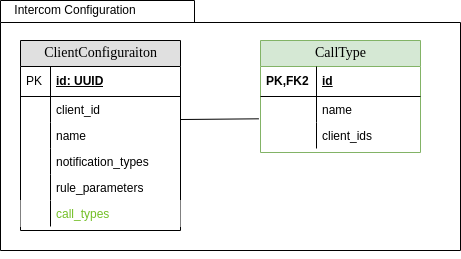
\includegraphics[width=\textwidth]{/home/joshua/FHNW/dev/IP6/IP6_Bachelorarbeit_Bericht_Cloudbasiertes_Praxisrufsystem/src/graphics/diagramms/erd_intercom_v02.drawio}
        \caption{ERD Ausschnitt - Konfiguration Gegensprechanlage}
    \end{minipage}
\end{figure}

Das Admin UI wird mit Ansichten erweitert, um CallTypes zu erstellen, anzeigen, bearbeiten und löschen.
Gleichzeitig wird der Cloudservice um Rest Endpunkte für das Lesen, Erstellen, Aktualisieren und Löschen von CallTypes erweitert.
Die Ansichten für ClientConfigurations im Admin UI werden so erweitert, dass CallTypes darauf angezeigt, hinzugefügt und entfernt werden können.
Die bestehenden Endpunkte für ClientConfiguration werden entsprechend erweitert.

\clearpage

\subsubsection{Signaling Instanz}

Mit WebRTC werden Peer To Peer Sprachverbindungen aufgebaut.\footnote{citation}
Bevor die Verbindung aufgebaut ist, kennen die beiden Clients sich gegenseitig noch nicht.
Die beteiligten Clients müssen Signale austauschen können um sich auf die Details der Verbindung zu einigen.
Es braucht deshalb eine Instanz, welche beide Seiten kennt und Vermittlung von Signalmeldungen übernimmt.
In Praxisruf übernimmt der Cloudservice die Funktion, Benachrichtigungen zu vermitteln.

Prinzipiell ist es möglich, den Signalaustausch in dieses Modul zu integrieren.
Dieser Ansatz hat aber zwei grosse Probleme.
Erstens ist die Grösse von Medlungen, welche über den gewählten Messaging Service (Firebase Cloud Messaging) ausgetauscht werden können beschränkt.
Meldungen zum Aufbau von WebRTC Verbindungen können diese Grösse überschreiten.\footnote{cite}
Zweitens geschieht das Versenden von Benachrichtigungen über einen asynchronen Mechanismus.
Die Signale für Sprachverbindungen sollen aber synchron ausgetauscht werden.
Es soll unmittelbar beim Versuch des Verbindungsaufbau klar sein, ob die Verbindung etabliert werden kann oder nicht.

Mit diesem Projekt wird der Cloudservice deshalb um ein weiteres Modul ''Signaling'' erweitert, welches den austausch von Signalen zwischen Clients ermöglicht.
Gleich wie das Modul für Sprachsynthese wird er unabhängig von den anderen Domänenmodulen im Cloudservice implementiert.
Alle Informationen, welche aus anderen Domänen benötigt werden, werden über Rest-Schnittstellen bezogen.
Das Modul Signaling übernimmt drittens Aufgaben.
Erstens muss es den Clients die Möglichkeit bieten, sich für Sprachverbindungen zu registrieren und diese Registrierungen verwalten.
Zweitens muss es Signalmeldungen empfangen und an die relevanten Empfänger zustellen.
Drittens muss es wann immer möglich Clients über nicht zustellbare Signale benachrichtigen.
Diese drei Funktionen müssen unabhängig von der gewählten Technologie für den Signalaustausch unterstützt werden.
Es wird ein entsprechendes Interface spezifiziert\footnote{Siehe Listing 6}.
Dieses definiert die Methoden afterConnectionEstablished und afterConnectionClosed.
Die beiden Methoden werden aufgerufen, wenn eine Verbindung geöffnet resp. geschlossen wurde.
Geöffnete Verbindungen werden in Memory geführt.
Dabei wird jede Verbindung durch eine UUID identifiziert.
Diese UUID entspricht der technischen Identifikation des entsprechenden Mobile Clients und muss, wenn sich der Mobile Client für eine Verbindung registriert mitgesendet werden.
Ein Mobile Client ist für den Signalaustausch verfügbar, wenn das Signaling Modul eine Verbindung mit seiner technischen Id kennt.
Sobald eine Verbindung geschlossen wurde, wird sie aus der Liste der in Memory Verbindungen wieder gelöscht.
Der entsprechende Mobile Client steht damit nicht mehr für den Signalaustausch zu Verfügung.

Für das Zustellen von Signalen wird die Methode sendMessage definiert.
Jede Message beinhaltet eine Payload und die Identifikation des Empfängers.
Der Signaling Service durchsucht die bekannten Verbindungen und findet die Verbindung für die Identifikation des Empfängers.
Anschliessend sendet er das Signal über die Verbindung dieses Empfängers.

Für die Verwaltung von bestehenden Verbindungen wird die Komponente ConnectionRegistry implementiert.
Diese muss Verbindungen anhand einer id registrieren und Verbindungen wieder entfernen können.
Weiter müssen Verbindungen anhand ihrer id gefunden werden können.
Die ConnectionRegistry wird als Wrapper um eine Java HashMap implementiert.
Durch die Verwendung der Map über einen Wrapper bleibt die Implementation aber unabhängig davon und kann leicht ausgetauscht werden. \footnote{Siehe Listing 7}

\clearpage

%\lstinputlisting[caption=ClientConnector.java,language=java,label={lst:ClientConnector.java}]{listings/ClientConnector.java}
%\lstinputlisting[caption=ClientConnector.java,language=java,label={lst:ClientConnector.java}]{listings/ConnectionRegistry.java}

\begin{figure}[h]
    \centering
    \begin{minipage}[b]{1\textwidth}
        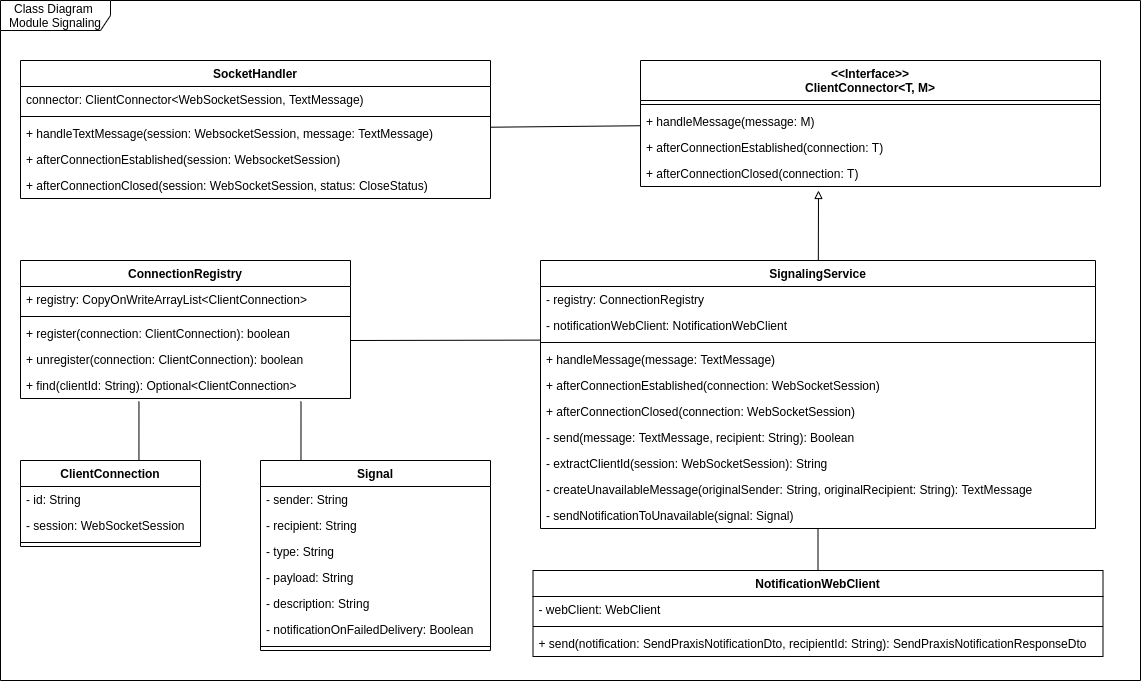
\includegraphics[width=\textwidth]{/home/joshua/FHNW/dev/IP6/IP6_Bachelorarbeit_Bericht_Cloudbasiertes_Praxisrufsystem/src/graphics/diagramms/Class_Intercom_Full_V01}
        \caption{Klassendiagramm SpeechSynthesisController}
    \end{minipage}
\end{figure}

Die Schnittestelle des Signaling Servers nach aussen wird mit Websockets umgesetzt.
Wie die restlichen Module des Cloudservices wird auch der Singaling Server als Spring Boot Modul umgesetzt.
Mit dem Projekt Spring-Boot-Starter-Websocket, können Websocketanbindungen in einer Spring Boot Applikation umgesetzt werden.\footnote{cite}
Es wird ein WebsocketHandler implementiert, welcher unter dem Pfad ''server-url/signaling'' erreichbar ist.
Die Implementation der Websocketschnittstelle implementiert das oben beschriebene ClientConnector Interface mit der entsprechenden Funktion.

Etablierte Verbindungen müssen eindeutig einem Client zugeordnet werden können.
Diese Client Identifikation wird als Query Parameter bei Verbindungsaufbau mitgegeben und im WebsocketHandler ausgelesen.
Anschliessend wird die WebsocketSession zusammen mit der Client Identifikation in der ConnectionRegistry gespeichert.
Wird die WebsocketSession geschlossen, wird sie durch den WebsocketHandler wieder von aus der ConnectionRegistry entfernt.

Der Zugriff auf den Signaling Service darf nur für Berechtigte möglich sein.
Um dies sicherzustellen, wird der Verbindungsaufbau nur erlaubt, wenn die Anfrage dazu authentisiert ist.
Für die Authentisierung wird derselbe Meachnismus wie für Http Anfragen in den anderen Cloudservice Domänen verwendet werden.
Über die SecurityConfig des Cloudservices wird die Authentification aller Http Requests überprüft.
Diese Konfiguration sorgt dafür, das unauthentifizierte Http Requests eine entsprechende Response erhalten.
Sie verhindert allerdings nicht, dass eine Websocketverbindung aufgebaut wurde, obwohl der Request nicht authentifiziert werden konnte.
Um dies zu verhindern, muss der Http Request für den Aufbau einer Websocketverbindung notwendig sind abgefangen werden und geprüft werden, ob der Request authentifiziert wurde.\cite{cite}
Spring bietet dazu die Klasse HttpSessionHandshakeInterceptor.
Mit der Methode beforeHandshake kann der Request vor dem Verbindungsaufbau abgefangen werden und die Authentisierung überprüft werden.
Ist diese gültig, wird die Verbindung aufgebaut.
Andernfalls wird der Verbindungsaufbau abgebrochen und eine Reponse mit HttpStatue ''unauthorized'' zurückgesendet.

\clearpage

\subsubsection{Anmeldung und Registrierung}

Der Ablauf von Anmeldung und Registrierung funktioniert mit dem neuen nativen Mobile Client grundsätzlich gleich wie zuvor.
Praxismitarbeitende öffnen die Applikation und geben ihr Benutzername und Passwort ein.
Der Mobile Client verwendet diese um sich über Basic Authentication beim Cloudservice anzumelden.
Als Antowrt auf die Anmeldung gibt der Cloudservice ein JWT Token zurück.
Dieses wird für die Authentifizierung aller weiteren Anfragen an den Cloudservice verwendet.
Nachdem die Anmeldung erfolgt ist, wird eine Liste aller Clientconfigurations die dem aktuellen Benutzer zur Verfügung stehen beim Cloudservice angefragt.
Der Benutzer wählt die gewünschte Konfiguration aus und bestätigt.

\begin{figure}[h]
    \centering
    \begin{minipage}[b]{0.9\textwidth}
        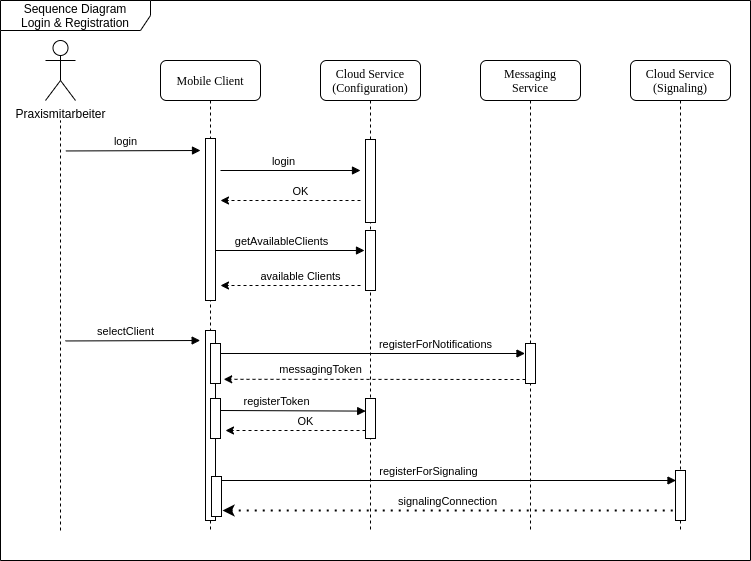
\includegraphics[width=\textwidth]{/home/joshua/FHNW/dev/IP6/IP6_Bachelorarbeit_Bericht_Cloudbasiertes_Praxisrufsystem/src/graphics/diagramms/Sequence_Registration}
        \caption{Mockup Home}
    \end{minipage}
\end{figure}

Danach wird diese Konfiguration geladen und die Hauptansicht angezeigt.
Die geladene Konfiguration beinhaltet alle Informationen die nötig sind um Buttons für Benachrichtigungen und Sprachverbindungen anzuzeigen.
Im Hintergrund muss sich der Mobile Client nun für Benachrichtigungen und Sprachverbindungen registrieren.
Für Benachrichtigungen registriert er sich zuerst beim Messaging Service.
Er erhält ein Token, welches den Client beim Messaging Service identifiziert.
Dieses Token sendet der Mobile Client zusammen mit der gewählten Konfiguration an den Cloudservice.
Dieser persistiert die Registrierung bei sich und kann sie verwenden um Benachrichtigungen an diesen Client zuzustellen.
Für Sprachverbindungen muss zudem eine Verbindung zum Signlaing Modul des Cloudservices aufgebaut werden.
Dazu wird wie in Kapitel 5.4.5 beschrieben eine Websocketverbindung geöffnet.

\clearpage
\subsubsection{Signalmeldungen}

Dieses Kapitel beschreibt die Signalmeldungen, welche für Sprachverbindungen verwendet werden.

\begin{figure}[h]
    \centering
    \begin{minipage}[b]{0.4\textwidth}
        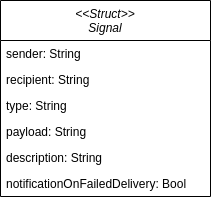
\includegraphics[width=\textwidth]{graphics/diagramms/Class_Signal_V01}
        \caption{Signal (Mobile Client)}
    \end{minipage}
\end{figure}

Alle Signalmeldungen beinhalten Identifikation von Sender und Empfänger.
Diese werden vom Signalingserver verwendet, um die Signale korrekt weiterzuleiten.
Type, Payload und Description werden im Mobile Client verwendet, um das Signal korrekt zu verarbeiten und Verbindungen aufzubauen.
Das Flag notificationOnFailedDelivery wird im Cloudservice ausgewertet.
Wenn ein Signal nicht zugestellt werden kann und dieses Flag TRUE ist, wird der Empfänger mit einer asynchrone Benachrichtigung darüber informiert.
Dazu wird das bestehende Notification Modul des Cloudservices verwendet.
Für die Verwaltung von Sprachverbindungen werden insgesamt sechs Typen von Signalmeldungen definiert.


\clearpage

Praxismitarbeitende können Sprachverbindungen zu anderen Clients aufbauen indem sie auf den entsprechenden Button in der Praxisruf App tippen.
Zum Zeitpunkt an dem der Button getippt wird, weiss der Mobile Client noch nicht, zu welchen Clients diese Verbindung aufgebaut werden soll.
Als erstes muss deshalb beim Cloudservice angefragt werden, welche Clients mit dem betätigten Button angesprochen werden sollen.
Der Cloudservice bietet dazu einen Endpoint an über den der vollständige CallType des verwendeten Buttons hinterlegt sind geladen werden können.
Nachdem diese Informationen geladen sind, können Sprachverbindungen zu allen relevanten Clients aufgebaut werden.
Dazu müssen Offer, Answer und Ice Candidate Signale ausgetauscht werden.
Der auslösende Client initialisiert die Peer to Peer Verbindung auf seiner Seite und sendet für jeden Gesprächspartner ein Offer.
Der Cloudservice findet die Verbindung der relevanten Empfänger und leitet die Signale über die jeweilige Verbindung weiter.
Die Verbindung auf Empfängerseite wird nach Eingang des Offers initialisiert.
Danach wird eine Answer zurück an den Initiator gesendet, welche über den Signalingserver zugestellt wird,
Der Initiator empfängt die Antwort Signale und ergänzt die notwendigen Verbindungsinformationen.
Folgende Graphik visualisiert diesen Ablauf:
\textbf{TODO: } Add ICE Candidate Exchange

\begin{figure}[h]
    \centering
    \begin{minipage}[b]{0.9\textwidth}
        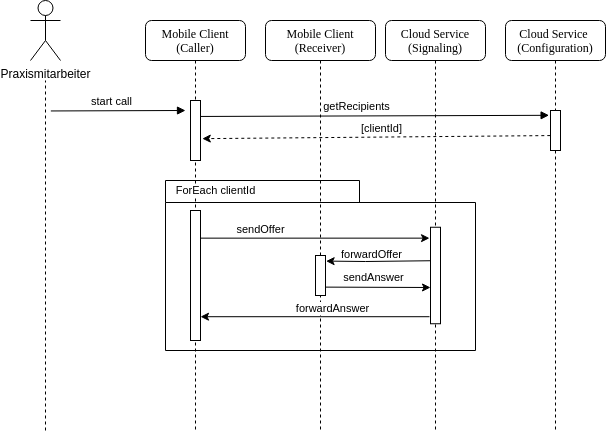
\includegraphics[width=\textwidth]{graphics/diagramms/Sequence_Intercom_Broking_V02}
        \caption{Ablauf Verbindungsaufbau Gegensprechanlage}
    \end{minipage}
\end{figure}

Nachdem die Offer und Answer Meldungen ausgetauscht sind, müssen Ice Candidate Meldungen versendet werden.
So können sich die CLients über Routing- und Protokollinformationen einigen die für die Peer to Peer Verbindung verwendet werden.
Der Austausch von Ice Meldungen wird in obiger Graphik nicht angezeigt.
Er verläuft nach demselben Prinzip wie der Austausch von Offer und Answer.
Sobald sich die Clients auf die Verbindungsinformationen geeinigt haben, besteht die Sprachverbindung.

\clearpage

\subsubsection{Anbindung Mobile Client an Singaling Server}

Für den Aufbau von Sprachverbindungen zwischen Mobile Clients müssen mehrere Signalmeldungen ausgetauscht werden.
Der Cloud Service wird im Rahmen dieses Projektes um eine Websocket Schnittstelle erweitert, welche dies ermöglicht.\footnote{Vgl. Kapitel 5.4}
Als Technologie für diese Schnittstelle werden Websockets verwendet.
Der Api Service wird dementsprechend erweitert, um Websocket Verbindungen zu ermöglichen.
Dies beinhaltet den Auf- und Abbau von Websocket Verbindungen, sowie das Senden und Empfangen von Meldungen über diese Verbindung.
Weiter muss die Verbindung konstant offen gehalten und im Fehlerfall erneut aufgebaut werden können.

Der Austausch von Signalmeldungen ist der einzige Anwendungsfall in Praxisruf, der Websocketverbindungen benötigt.
Deshalb wird auf eine generische Integration von Verbindungen analog von Http Verbindungen\footnote{Vgl. Kapitel 5.2.2} verzichtet.
Stattdessen wird eine Extension Klasse PraxisrufApi+Signaling nach folgendem Muster erstellt:

\begin{figure}[h]
    \centering
    \begin{minipage}[b]{0.9\textwidth}
        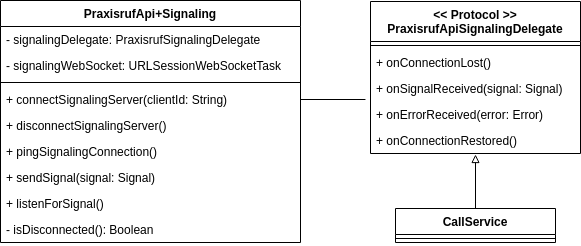
\includegraphics[width=\textwidth]{graphics/diagramms/Class_Mobile_Client_Signaling_Connection}
        \caption{Klassendiagramm - Signaling Schnittstelle in Mobile Client}
    \end{minipage}
\end{figure}

Die Signaling Extension kann immer genau eine offene Verbindung verwalten.
Diese wird als Instanzvariable innerhalb des Services geführt.
Der Status dieser Verbindung kann als Computed Property "disconnected" intern abgefragt werden.
Die Extension bietet Methoden um den Signaling Service zu Verbinden.
Eine Verbindung wird dabei immer spezifisch für die aktuell gewählte Client Configuration geöffnet. \footnote{Vgl. Kapitel X.X}
Weiter werden Methoden angeboten, um Pingsignale zu senden oder die Verbindung zu trennen.
Zudem bietet die Extension Methoden, um Signalmeldungen über die geöffnete Verbindung zu senden,
sowie eine Methode um empfangene Signalmeldungen zu verarbeiten.
Für die Integration der Singalingverbindung in den Rest der Applikation, wird das Protokoll PraxisrufApiSignalingDelegate definiert.

Vor dem Versenden einer Signal- oder Pingmeldung wird überprüft, ob eine Verbindung geöffnet und Fehlerfrei ist.
Ist dies nicht der Fall, wird die Verarbeitung die onConnectionLostMethode des Delegates aufgerufen.
Die Implementation dieses Delegates ist dafür verantwortlich, die Verbindung wieder zu öffnen.
Die Methoden onSignalReceived resp. onErrorReceived werden aufgerufen wenn ein Signal resp. eine Fehlermeldung empfangen wurde.
Im Fehlerfall soll wenn nötig eine Fehlermeldung angezeigt werden und die Verbindung repariert werden.
Wenn eine Signalmeldung empfangen wurde, muss diese an die Applikation zu Verarbeitung weitergereicht werden.

\clearpage

\subsubsection{Signalverarbeitung im Mobile Client}

Neben austausch von Signalen muss auch die Sprachverbindung selbst verwaltet werden.
Die Details der Sprachverbindung sind vendor spezifisch.
Es wird deshalb eine eigene Klasse CallClient erstellt.
Diese ist für das Verwalten von Verbindungen verantwortlich.
Bei eingehenden Verbindungen muss sie signale empfangen, die Verbindung erstellen.
Wenn nötig Antowrt Signale erstellen und zurückgeben.
Bei ausgehenden Verbindungen muss sie Verbindung initialisieren.
Es muss Signal erstellt und versendet werden.
Weiter müssen Methoden angeboten werden um die Unterhaltung oder das Microphon zu muten.
Und um die Verbindung zu schliessen.
Und um den bei Änderung des internen Status, das UI entsprechend zu aktualisieren.

Um die Integration der Sprachverbindung möglichst unabhängig und auswechselbar zu machen, wird der CalLClient nicht direkt in der View verwendet.
Stattdessen definiert der CallClient ein Delegate Protocol, welches die notwendigen Callbacks definiert.

\begin{figure}[h]
    \centering
    \begin{minipage}[b]{0.9\textwidth}
        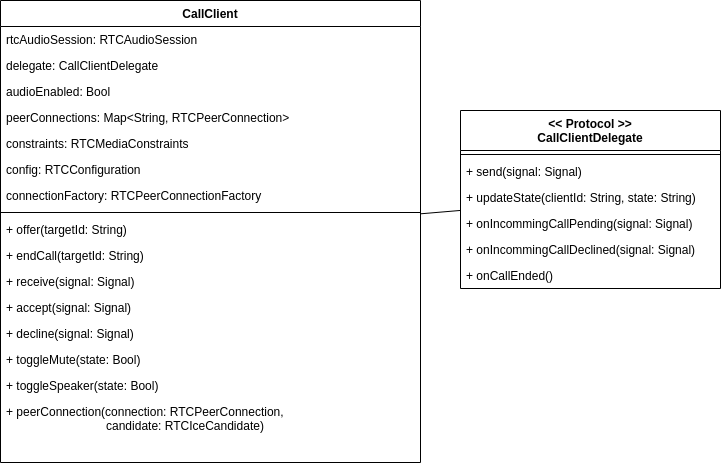
\includegraphics[width=\textwidth]{graphics/diagramms/Class_Mobile_Client_Signal_Processing}
        \caption{Klassendiagramm - Signalingverarbeitung in Mobile Client}
    \end{minipage}
\end{figure}

Um Anrufe in der Applikation verwenden zu können müssen CallClient und PraxisrufApi+Signaling in die Benutzeroberfläche integriert werden.
Beide Applikationen definieren ein Delegate Protocol, welches die Funktionen spezifiziert, über welche die Komponenten eingebunden werden können.
Es wird eine weitere Serviceklasse mit dem Namen CallService implementiert, welche beide Delegate Protocols implementiert.
Dieser Service instanziert CallClient und PraxisrufApi+Signaling und registriert sich anschliessend als Delegate bei beiden Instanzen.
Der CallService selbst wird in der View verwendet.
Er nimmt Benutzereingaben entgegen und delegiert die entsprechende Funktionalität an den CallClient und SignalingClient.

Wenn der Benutzer einen Anruf startet, wird die View für aktive Anrufe geladen.
Diese initialisiert den Anruf über den CallService.
Der CallService ruft dazu als erstes den CallClient auf.
Der CallClient initialisiert die lokalen Verbindungsinformationen und erstellt ein Signel, um den Empfänger zu informieren.
Dieses Signal gibt er an den CallService weiter.
Der CallService leitet das Signal an den SignalingClient weiter, welcher das Versenden an den Cloud Service übernimmt.

\clearpage
\begin{figure}[h]
    \centering
    \begin{minipage}[b]{0.8\textwidth}
        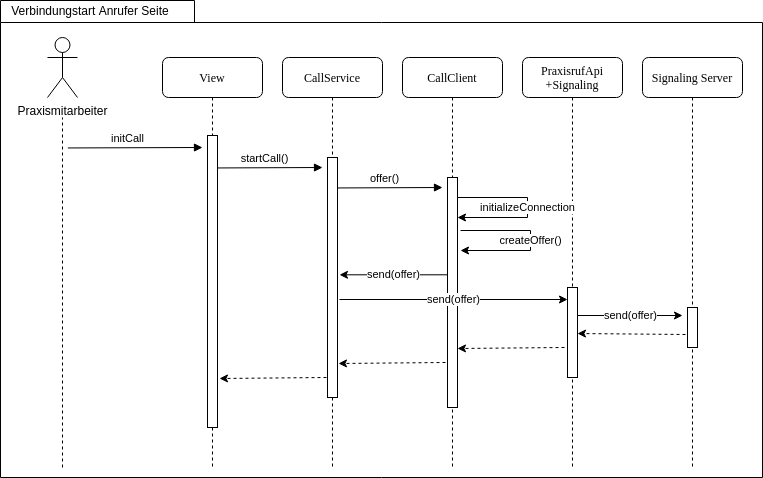
\includegraphics[width=\textwidth]{/home/joshua/FHNW/dev/IP6/IP6_Bachelorarbeit_Bericht_Cloudbasiertes_Praxisrufsystem/src/graphics/diagramms/Sequence_MobileClient_Caller_Signaling.drawio}
        \caption{MobileClient - Anruf Starten Signal}
    \end{minipage}
\end{figure}

Das versendete Signal wird über das Signaling Modul des Cloud Service an den Empfänger übermittelt.
Dieser empfängt das Signal über den SingalingClient.
Der SignalingClient gibt das Signal über onSignalReceived an den CallService weiter.
Der CallService aktiviert die Ansicht für aktive Anrufe und leitet das Signal an den CallClient weiter.
Der CallClient initialisiert die lokalen Verbindungsinformationen und erstellt eine Signal zur Bestätigung.
Dieses Signal wird wiederun über den CallService zum SignalingClient weiter zum Cloud Service versendet.
Auf Starterseite, kann diese Bestätigung weiterverarbeitet werden.

\clearpage

\subsubsection{Verpasste Anrufe}

Anrufe über die Gegensprechanlage können nur empfangen werden, solange die Praxisruf App im Vordergrund läuft und beim Signalingserver registriert ist.
Ist dies nicht der Fall, kann der Signalingserver keine Signale an den jeweiligen Empfänger zustellen.
Wenn der Singalingserver ein Signal für einen Empfänger erhält, der nicht verbunden ist wird versucht, diese über eine Benachrichtigung zu informieren.
Benachrichtigungen für verpasste Anrufe, werden gleich wie alle anderen Benachrichtigungen empfangen und in der Inbox angezeigt.
Für das Versenden der Benachrichtigung für verpasste Anrufe wird das bestehende Notification Modul des Cloudservice verwendet.
Dieses wird um einen Endpunkt erweitert, der es erlaubt Benachrichtigungen gezielt an einen einzelnen Client zu versenden.
Der neue Enpunkt nimmt zwei Parameter entgegen:
Die technische Identifikation des Empfängers und die technische Identifikation des relevanten Benachrichtigungstyps.
Der relevante Benachrichtigungstyp muss durch den Praxisadministrator im Admin UI erfasst werden.
Die technische Identifikation dieses Benachrichtigungstyps muss anschliessend in den Umgebungsvariablen des Signalingservices hinterlegt werden.\footnote{Vgl. Installationsanleitung}
Wenn der Empfänger nicht für Benachrichtigungen registriert ist, kann er nicht über den verpassten Anruf informiert werden.
Dasselbe gilt, wenn die Benachrichtigung aus technischen Gründen nicht zugestellt werden kann.
Im Rahmen dieses Projektes wird kein Mechanismus implementiert, um diese fehlgeschlagene Zustellung automatisch zu wiederholen.

\subsubsection{Deaktivierte Anrufe}

Praxismitarbeitende können das Empfangen von Anrufen lokal deaktivieren.
Wenn der Empfang von Anrufen deaktiviert ist, werden Offer Signale nicht mit einer Answer sondern mit einem Declined Signal beantwortet.
Empfängt ein Client ein Declined Signal, erstellt er lokal einen Eintrag in der Inbox und zeigt eine Push Benachrichtigung an um den Benutzer darauf hinzuweisen.

\subsubsection{Verbindungsende}

Praxismitarbeitende können Sprachverbindungen durch einen Button beenden.
Durch antippen des Auflagen-Buttons wird die bestehende Peer to Peer Verbindung zum Gesprächspartner getrennt.
Anschliessend wird ein Signal vom Typ End an die Gesprächspartner gesendet.
Durch Empfang des End-Signals, weiss der Gesprächspartner, dass die Verbindung durch das Gegenüber getrennt wurde und kann die Verbindung seinerseits entfernen.

\subsubsection{Security}

Der Austausch von Daten über Websockets erfolgt ausschliesslich über Secure WebSockets (WSS).
Für den Aufbau von Websocketverbindungen, muss der Benutzer ebenfalls authentifiziert sein.
Dazu muss der Http-Handshake Request um die Websocketverbindung zu öffnen mit einem entpsrechend gültigem JWT Token authentifiziert werden.


\clearpage
